\documentclass[11pt,a4paper]{article}
\usepackage[margin=2.2cm]{geometry}
\usepackage{amsmath,amssymb}
\usepackage{graphicx}
\usepackage{booktabs,multirow,array,tabularx,longtable}
\usepackage{xcolor}
\usepackage{xurl}
\usepackage[hidelinks]{hyperref}
\usepackage{enumitem}
\usepackage{caption}
\usepackage{float}
\captionsetup{font=small,labelfont=bf}
\setlist{itemsep=2pt,topsep=4pt}

\newcommand{\nue}{\ensuremath{\nu_e}}
\newcommand{\numu}{\ensuremath{\nu_\mu}}
\newcommand{\code}[1]{\texttt{\small #1}}
\newcommand{\best}[1]{\textbf{#1}}
\newcommand{\pft}{\ensuremath{^\dagger}}
\newcolumntype{L}{>{\raggedright\arraybackslash}X}

\title{\textbf{Charge + Light Foundation Model for MicroBooNE Open Data:\\ Comparison with Reference Algorithms}\\[4pt]
\large Technical Note --- Round 2}
\author{Haiwang Yu\thanks{Prepared with the assistance of Claude (Anthropic). Code: \url{https://github.com/HaiwangYu/fm4npp-lartpc}, branch \code{round2-references}, package \code{multi-modal-qlmatch/qlfm}. Tracking: GitHub issue \#3. Round 1 (the qlfm model itself, ablations and scaling) is described in \code{docs/technote-round1.pdf} and is not repeated here.}}
\date{October 20, 2026}

\begin{document}
\maketitle

\begin{abstract}
\noindent
We compare our multi-modal (TPC charge + PMT light) masked-autoencoder foundation model, qlfm, with two kinds of reference. The first is the reconstruction already shipped in the MicroBooNE open data: Pandora's own outputs, and a gradient-boosted classifier trained on Pandora features. The second is four published foundation-model recipes, adapted to the same data: FM4NPP, Panda, PoLAr-MAE, and a self-distillation variant inspired by Panda~v2.

All neural models get equal pretraining compute (about 4 node-hours each), identical task heads with identical late-fused light, and identical label budgets and test subsets. The downstream tasks are hit-level and event-level neutrino/cosmic separation, flavor classification, and energy regression.

With at least 1\% of labels (3--7k events), the 21M-parameter qlfm-M is the best method on all four tasks. With a frozen backbone it reaches event AUC 0.999, flavor macro-F1 0.71, energy resolution 0.28 and hit F1 0.89. The best other foundation model, Panda, reaches 0.978, 0.68, 0.34 and 0.72; the Pandora+BDT reference reaches 0.976, 0.63 and 0.34, and Pandora's $\nu$-slice hits reach F1 0.65.

With only 0.1\% of labels, the Pandora+BDT reference beats every frozen foundation model on flavor and energy.

A per-event analysis of 120 easy, boundary and hard events (Appendix~\ref{app:displays}) shows that the residual errors cluster in a few places:
\begin{itemize}
  \item at the label boundaries (out-of-active-volume neutrinos; NC versus \numu CC);
  \item at the tails of the energy spectrum;
  \item in events whose neutrino deposits only a few percent of the charge.
\end{itemize}
Round 2 used 38.7 Polaris node-hours.
\end{abstract}

\tableofcontents
\clearpage

%=====================================================================
\section{Summary of findings}
%=====================================================================
\begin{enumerate}[leftmargin=*]
\item \textbf{qlfm-M (multi-modal MAE, 21M) is the best method on all four tasks once $\geq$1\% of labels are available.} Frozen backbone, 1\% / 10\% labels:

\begin{center}\footnotesize
\begin{tabular}{lccc}
\toprule
Task (metric) & qlfm-M CL & best other FM (Panda) & Pandora+BDT (+light)\\
\midrule
T2 event $\nu$/cosmic (AUC) & \best{0.999 / 0.999} & 0.978 / 0.984 & 0.976 / 0.983\\
T3 flavor (macro-F1) & \best{0.713 / 0.755} & 0.679 / 0.734 & 0.632 / 0.655\\
T4 energy (resolution, lower better) & \best{0.284 / 0.276} & 0.343 / 0.302 & 0.342 / 0.308\\
T1 hit $\nu$/cosmic (charge-weighted F1) & \best{0.892 / 0.894} & 0.715 / 0.725 & 0.651 ($\nu$ slice)\\
\bottomrule
\end{tabular}
\end{center}

\item \textbf{With very few labels (0.1\%, about 260--720 events), Pandora+BDT is competitive.}
  \begin{itemize}
    \item It beats every \emph{frozen} foundation model on flavor (0.559 vs 0.531 for qlfm-M) and on energy (0.400 vs 0.418).
    \item Fine-tuning qlfm-M overtakes it (0.640 and 0.385).
    \item Low-dimensional reconstruction features are therefore a strong low-label prior.
    \item Pandora+BDT saturates early, at flavor 0.66 and energy 0.31 at 10\% labels.
  \end{itemize}

\item \textbf{Panda (PTv3 + Sonata self-distillation, size-matched to 21M) is the strongest external recipe and the best charge-only representation.}
  \begin{itemize}
    \item Without any light it still reaches T2 AUC 0.914, against 0.61--0.71 for the other charge-only backbones.
    \item It is the only reference whose per-hit features beat Pandora's $\nu$ slice (0.715 vs 0.651).
  \end{itemize}

\item \textbf{PoLAr-MAE and FM4NPP land between our small charge-only and charge+light models.}
  \begin{itemize}
    \item With late light both reach T2 AUC 0.96.
    \item Frozen, they fall below Pandora+BDT on flavor and energy, and below Pandora's $\nu$ slice on hits (0.54 and 0.46).
  \end{itemize}

\item \textbf{Light matters for every backbone.}
  \begin{itemize}
    \item The identical late-fused light head raises T2 from 0.61--0.91 (charge only) to 0.96--0.98.
    \item qlfm's early fusion, with light inside the backbone, goes further: 0.999.
  \end{itemize}

\item \textbf{Our self-distillation variant (qlfm-SD) underperforms MAE on the same backbone.} Frozen hit F1 is $\leq$0.15 and flavor about 0.45. The likely cause is a learning rate about 3$\times$ too low. Panda shows the objective itself works.

\item \textbf{Where the algorithms fail} (Sec.~\ref{sec:displays}):
  \begin{itemize}
    \item T2 errors concentrate on out-of-active-volume (out-of-AV) $\nu$: 832 of the 1{,}208 events that at most one algorithm gets right are out-of-AV.
    \item T3 errors are dominated by NC and \nue CC events called \numu CC.
    \item T4 failures sit in the tails of the energy spectrum, because every regressor pulls predictions toward the mean.
    \item T1 failures are events whose $\nu$ deposits only a few percent of the charge. Per event, qlfm-M reaches F1$_q\geq0.8$ in 79\% of events, against 51\% for Pandora's $\nu$ slice and $\leq$25\% for every other foundation model.
  \end{itemize}
\end{enumerate}

%=====================================================================
\section{Data, tasks and metrics}
%=====================================================================
All methods use the same corpus, splits, tasks and metrics as round~1.

\paragraph{Data.} The corpus combines the MicroBooNE open-data inclusive overlay (753k events) and the \nue{} overlay (77k), 830{,}807 events in total, in the HDF5 ``NoWire'' format: reconstructed wire hits, optical hits, Pandora tables and truth. It is split by (run, subrun) into train, val and test. Label pools \code{lab\_f0.001/0.01/0.1} are nested random subsets of the train split.

\paragraph{Tasks and metrics.}
\begin{description}[leftmargin=1.2em]
\item[T1 hit $\nu$/cosmic.] A hit is $\nu$ if its true $\nu$ energy deposit exceeds 0.05\,MeV. Metric: charge-weighted F1 (F1$_q$) at threshold 0.5, over 3{,}000 test events.
\item[T2 event $\nu$ presence.] Three classes:
  \begin{itemize}
    \item 0, no-$\nu$: $\leq$5 $\nu$ hits;
    \item 1, visible in-AV $\nu$: vertex inside the active volume and $\geq$30 collection-plane $\nu$ hits;
    \item 2, out-of-AV $\nu$: more than 5 $\nu$ hits otherwise.
  \end{itemize}
  Headline metric: AUC of class 1 versus class 0.
\item[T3 flavor.] \numu CC, \nue CC or NC, for events with a visible $\nu$ whose vertex is inside the fiducial volume (AV minus 3\,cm). Metric: macro-F1.
\item[T4 energy.] Regression of $\log E_\nu$ for CC events with a visible $\nu$ and a fiducial vertex. Resolution is half the 16--84\% width of $E_\text{pred}/E_\text{true}-1$; lower is better.
\begin{itemize}
  \item \textbf{$E_\nu$ is the true energy of the incoming neutrino} (generator truth, column \code{nu\_energy} of \code{event\_table}). It is \emph{not} the deposited or visible energy.
  \item A large part of it is never seen as charge: exiting muons, neutrons, nuclear binding, and energy below threshold. The $\nu$'s MC energy deposited on collection-plane hits is a median 47\% of $E_\nu$: 44\% for \numu CC, which often has exiting muons, and 57\% for \nue CC.
  \item A log-linear calibration of that \emph{true} deposited energy to $E_\nu$ reaches only 0.36 resolution on the same test events. This is an oracle for pure calorimetry with perfect $\nu$/cosmic separation.
  \item The best models do better (0.28), so they also use topology: track lengths, containment and event type.
  \item Pandora direct calibrates the summed collection charge of its $\nu$ slice to $\log E_\nu$ in the same way.
\end{itemize}
\end{description}
Test subsets for T2--T4 are 10{,}000 events drawn with a fixed seed. The Pandora references (Sec.~\ref{sec:pandora}) were scored on a 20{,}000-event superset drawn from the same permutation.

%=====================================================================
\section{Algorithms and parameters}\label{sec:algs}
%=====================================================================
\subsection{Pandora references (no neural network)}\label{sec:pandora}
\paragraph{Pandora direct.} Uses the reconstruction stored in the open-data HDF5 files as is. The ``best $\nu$ slice'' is the \code{pandoraPrimary} slice with the highest \code{nu\_score}.
\begin{center}\small
\begin{tabularx}{\textwidth}{lL}
\toprule
Task & Pandora-direct prediction\\
\midrule
T1 & Hits in the best $\nu$ slice are $\nu$.\\
T2 & Score = best \code{nu\_score} clipped to $[-1,1]$, or $-1$ if there is no slice. AUC from the score. For the event displays (3-class), score $>0.5$ means class 1, else class 0. Pandora has no ``out-of-AV'' output.\\
T3 & Best-slice \code{slice\_pdg}: 14 $\to$ \numu CC, 12 $\to$ \nue CC, anything else (including no slice) $\to$ NC.\\
T4 & Calorimetric: $\log E = a + b\cdot\log(1+\sum q_Y)$, where $\sum q_Y$ is the summed collection-plane charge of the best slice. $a$ and $b$ come from a linear fit on all eligible \emph{training} events, so this calibration uses 100\% of labels.\\
\bottomrule
\end{tabularx}
\end{center}

\paragraph{Pandora + BDT.} A classic ``reconstruction + ML'' analysis baseline. Its features are 32 charge features plus, in the ``+light'' variant, 8 summary features of the largest beam flash (Table~\ref{tab:bdtfeat}). It is trained on exactly the same label pools as the neural models.
\begin{center}\small
\begin{tabularx}{\textwidth}{lL}
\toprule
Parameter & Value\\
\midrule
Model & scikit-learn \code{HistGradientBoostingClassifier(class\_weight="balanced")} (T2, T3); \code{HistGradientBoostingRegressor} with squared error on $\log E$ (T4)\\
Boosting & \code{max\_iter} 500, learning rate 0.1, early stopping on 15\% of the label pool, patience 20\\
Trees & 31 leaves max, \code{min\_samples\_leaf} 20, no L2, 255 bins (library defaults)\\
Training sets & \code{lab\_f} 0.001 / 0.01 / 0.1 / 1.0 $\cap$ task eligibility; the same $n_\text{train}$ as the neural runs (e.g.\ T3: 325 / 3{,}211 / 31{,}794 / 316{,}838)\\
Seeds & 0, 1, 2 for label fractions $\leq$1\%; 0 otherwise\\
\bottomrule
\end{tabularx}
\end{center}

\begin{table}[H]\centering\small
\caption{Pandora+BDT input features (per event; ``best slice'' as above).}\label{tab:bdtfeat}
\begin{tabularx}{\textwidth}{lL}
\toprule
Group & Features\\
\midrule
Slices (6) & number of slices; number of $\nu$-like slices; best \code{nu\_score}; best slice is \nue-like or \numu-like (2); $\log(1+\text{flash-match score})$\\
Vertex (4) & best-slice vertex $x,y,z$; vertex inside the AV\\
PFPs (6) & PFP, track and shower counts; max / min / mean track--shower score\\
Hits (12) & best-slice hit count and $\log\sum q$ on U, V, Y; PFP-associated hit count and $\log\sum q$ on U, V, Y\\
Extents (4) & collection-plane time span and wire span; charge-weighted $z$; mean time\\
\midrule
Light (8) & number of flashes; $\log(1+\text{PE})$, time, PE-weighted $z$ and $y$ centroid, $z$ RMS and number of lit PMTs of the largest beam flash; slice--flash $\Delta z$\\
\bottomrule
\end{tabularx}
\end{table}

\subsection{qlfm-S / qlfm-M: multi-modal masked autoencoder (ours)}
\begin{itemize}
  \item \textbf{Tokens.} Charge hits are grouped into occupied (plane, 16-wire $\times$ 64-tick) cells; each cell becomes one token, positioned at its charge centroid. Each event also gets 32 PMT tokens, one per PMT, carrying its time profile.
  \item \textbf{Encoder.} A pre-LN Transformer attends jointly over charge and light tokens (early fusion).
  \item \textbf{Pretraining.} Masked autoencoding: a light decoder reconstructs the sub-cell charge pattern of masked charge tokens and the time profile of masked PMTs.
\end{itemize}
\begin{center}\small
\begin{tabular}{lcc}
\toprule
Parameter & qlfm-S CL & qlfm-M CL\\
\midrule
Width / depth / heads & 256 / 8 / 8 & 384 / 12 / 6\\
Backbone parameters & 6.58M & 21.79M\\
Steps (events seen) & 17k (4.35M) & 34k (8.70M)\\
Pretraining node-hours & 0.72 & 2.05\\
\bottomrule
\end{tabular}\\[6pt]
\begin{tabularx}{\textwidth}{lL}
\toprule
Shared setting & Value\\
\midrule
Block & pre-LN; FlashAttention-2 varlen (bf16); MLP ratio 4; GELU; no dropout or drop-path\\
Charge token & cell of 16 wires $\times$ 64 ticks; at most 4{,}096 per event in pretraining, 8{,}192 downstream\\
Per-hit features & in-cell offset (2), $\log(1+q/200)$, rms/5 $\to$ MLP 4--64--128 (128-d hit embedding)\\
Cell embedding & PointNet max $\Vert$ mean $\Vert$ (log $n_\text{hit}$, log $\sum q$) $\to$ MLP; plane embedding\\
Position & Fourier features (10 frequencies) of the charge centroid (drift cm, wire cm) + MLP(in-cell offset)\\
Light token & 32 per event; $\log(1+\text{PE})$ in 16 time bins (0--24\,$\mu$s) + total; Fourier(PMT $y,z$) + PMT-ID\\
Charge masking & 60\%: half as cross-plane drift strips (256 ticks, $p=0.3$), the rest random\\
Light masking & per event: 40\% all PMTs, 40\% half of the PMTs, 20\% none\\
Decoder & width 192, 3 layers, 6 heads, learnable mask tokens\\
Targets / loss & charge: 4$\times$8 sub-cell $\log\sum q$ + 2 statistics, standardized; light: 17-d profile; MSE$_q$ + 1.0 MSE$_L$\\
Data & full train split (747k events), 4 GPUs $\times$ 64 = 256 events/step\\
Optimizer & AdamW $\beta=(0.9,0.95)$, wd 0.05, lr $1.5\times10^{-4}$, 5\% warmup + cosine, clip 1.0, bf16\\
\bottomrule
\end{tabularx}
\end{center}
qlfm-S C is identical to qlfm-S CL but has no light tokens.

\subsection{qlfm-SD: self-distillation on qlfm tokens (Panda~v2-inspired)}
Panda~v2~\cite{pandav2} has no public code, and its key hyperparameters are unpublished. We therefore test Panda-style self-distillation on the qlfm-M backbone instead, applying v2's hint to drop masked tokens and distil only the observable ones. The EMA teacher is the backbone used downstream.
\begin{center}\small
\begin{tabularx}{\textwidth}{lL}
\toprule
Parameter & Value\\
\midrule
Backbone & as qlfm-M (384 / 12 / 6, 21.79M), light tokens inside\\
Views & 2 global (drift window covering 40--100\% of the event's time span, masked, with light); 6 local (10--40\%, unmasked, no light)\\
Masking & ratio 0.5 $\to$ 0.9 over the first 5\%; half 256-tick strips, half random; masked tokens dropped\\
Head & MLP $d$--2048--2048--256, $\ell_2$-normalized $\to$ 4{,}096 weight-normalized prototypes\\
Teacher & EMA 0.994 $\to$ 1 (cosine); sees the full event; Sinkhorn--Knopp (3 iterations); temperature 0.04 $\to$ 0.07; student temperature 0.1\\
Loss & cross-entropy on observed tokens; weight 0.5 split over the global views and 0.5 over the local views\\
Optimization & 4 GPUs $\times$ 8 events; 61{,}922 steps (fixed by a 3.47\,h budget; 1.98M events); AdamW (0.9, 0.95), wd 0.05; lr $1.875\times10^{-5}$ (MAE batch scaling, about 3$\times$ below usual DINO scaling); clip 1.0; bf16\\
Pretraining & $\approx$3.7 node-hours\\
\bottomrule
\end{tabularx}
\end{center}

\subsection{FM4NPP port~\cite{fm4npp}}
FM4NPP is a causal Mamba2 sequence model over individual detector hits. It is pretrained by $k$-nearest-next-neighbour (k-NNN) regression. We ported the released \code{MambaGPT} to \code{mamba\_ssm}~2.2.5.

Three deviations were forced by 2D wire data:
\begin{itemize}
  \item hits are serialized in a time-major raster;
  \item neighbours are restricted to the same plane;
  \item targets are \emph{relative} in-plane offsets. Absolute coordinates were solved almost trivially by copying the input: loss 0.004 after 75 steps.
\end{itemize}
\begin{center}\small
\begin{tabularx}{\textwidth}{lL}
\toprule
Parameter & Value\\
\midrule
Architecture & $d=256$, 12 blocks of $x + \text{Dropout}_{0.1}(\text{Mamba2}(\text{RMSNorm}(x)))$; d\_state 16, d\_conv 4, expand 2, head dim 64; 4.90M parameters (the published ``m3'' size)\\
Input embedding & fixed random projection of $\log$-charge + fixed random projection of NeRF features (10 frequencies) of (wire/$N_\text{wire}$, tick/6400, plane/2)\\
Serialization & 1 token per hit, at most 16{,}384 per event; sort by 8 drift slabs $\to$ plane $\to$ 8 wire boxes $\to$ wire $\to$ tick\\
Objective & $k=30$ nearest same-plane hits later in the sequence; regress (wire cm, drift cm) offsets / 10\,cm; MSE; fp32 linear head 256 $\to$ 60\\
Optimization & 4 GPUs $\times$ 8 events (about 115k tokens/GPU); 64k steps (2.05M events, about 30G tokens); AdamW (0.9, 0.95), lr $2\times10^{-4}$, wd 0.01, 10\% warmup + cosine, clip 0.1; bf16\\
Downstream features & softmax-weighted mix of all 12 layer outputs (trainable \code{adapter\_mix}) + LayerNorm, per hit\\
Pretraining & 3.62 node-hours\\
\bottomrule
\end{tabularx}
\end{center}

\subsection{Panda~\cite{panda}}
Panda is a Sonata-style~\cite{sonata} self-distillation of a Point Transformer~V3 on sparse point clouds. We use the \code{pimm} implementation. Each plane of each event is one 2D point cloud, with points at (wire$\times$0.3\,cm, drift cm, plane$\times$10\,cm) and energy equal to the hit integral.
\begin{center}\small
\begin{tabularx}{\textwidth}{lL}
\toprule
Parameter & Value\\
\midrule
Model & Sonata-v1m1 + PT-v3m2 encoder; depths (2,2,2,4,2), channels (32,64,128,256,320), heads (2,4,8,16,20), patch 256, strides 2; serializations Hilbert, Hilbert-transposed, Z, Z-transposed (shuffled); student drop-path 0.3; 20.57M backbone (size-matched; published 91M)\\
Input & 4 channels (normalized $x,y,z$; log energy); grid 0.3\,cm; NormalizeCoord centre (520, 130, 10)\,cm, scale 600; LogTransform 10--5000\\
Views / augmentation & 2 global (40--100\%) + 6 local (10--40\%) crops, at most 30k points; in-plane rotation, flips, jitter, scale [0.9, 1.1], energy jitter 5\%\\
Masking & patch 2 $\to$ 15\,cm; ratio 0.5 $\to$ 0.9 (5\% warmup)\\
Head & up-cast 2 levels (704-d) $\to$ MLP 4096 $\to$ 256 $\to$ 4{,}096 prototypes; Sinkhorn--Knopp; teacher temperature 0.04 $\to$ 0.07; student 0.1; EMA 0.994 $\to$ 1; loss weights mask 2/8, roll-mask 2/8, unmask 4/8\\
Optimization & batch 64 clouds (16/GPU); 1.84M clouds once (28{,}750 iterations, 0.44\,s each); AdamW base lr $3.0\times10^{-3}$ with block-wise decay 0.9; wd 0.04 $\to$ 0.2; OneCycle (5\%, cosine); clip 3.0; bf16\\
Downstream features & teacher backbone, up-cast to the 0.3\,cm voxels (704-d); each hit takes its voxel's feature\\
Pretraining & $\approx$3.7 node-hours\\
\bottomrule
\end{tabularx}
\end{center}

\subsection{PoLAr-MAE~\cite{polarmae}}
PoLAr-MAE is a masked point-cloud autoencoder. A ViT encodes point groups ``patches'', and the model reconstructs the positions and energies of masked groups. It uses the same plane clouds as Panda.
\begin{center}\small
\begin{tabularx}{\textwidth}{lL}
\toprule
Parameter & Value\\
\midrule
Encoder & ViT-S: 384-d, 12 layers, 6 heads, post-norm, position added at every layer, attention dropout 0.05, drop-path 0.25; 21.3M (decoder 384-d $\times$ 4 layers, 7.1M; total 29.0M)\\
Tokenizer & farthest-point sampling of 2048 candidates $\to$ C-NMS (overlap 0.72) $\to$ at most 1{,}024 groups per cloud; ball radius \textbf{4\,cm} (published 1.5\,cm); 32 points per group; mini-PointNet embedding\\
Objective & 60\% random group masking; Chamfer + per-point energy loss (weights 1, 1)\\
Optimization & batch 64 clouds; 1.67M clouds $\times$ 3 passes (78{,}281 iterations, 0.16\,s each); AdamW lr $4\times10^{-4}$, wd 0.05; OneCycle (5\%, cosine); clip 3.0; fp32\\
Downstream features & encoder without masking; each hit takes the token of the nearest group centre\\
Pretraining & $\approx$3.7 node-hours\\
\bottomrule
\end{tabularx}
\end{center}
The 4\,cm radius is needed because a 10\,m $\times$ 3.5\,m plane with about 26 cosmic tracks would need about 2k groups at 1.5\,cm.

\subsection{Common downstream interface and protocol (R2P)}
Every backbone exposes token features $z$, an event index, and a hit-to-token map (plus a 128-d hit embedding for qlfm). Identical heads sit on top:
\begin{itemize}
  \item \textbf{AttnPool} (T2--T4): LayerNorm, then 4 learned queries $\times$ 8 heads over all tokens of the event, then an MLP $4d$--256--$n_\text{out}$.
  \item \textbf{HitHead} (T1): [hit embedding (qlfm only) $\Vert$ LN(token feature of the hit) $\Vert$ pooled light] $\to$ MLP 128--128--1.
  \item \textbf{LateLight}: the qlfm PMT embedding (32 tokens per event), added to the pooled token set (T2--T4) or the hit feature (T1) of \emph{every} backbone. qlfm-CL also has light inside the backbone (early fusion).
\end{itemize}
\begin{center}\small
\begin{tabularx}{\textwidth}{lL}
\toprule
Parameter & Value\\
\midrule
Modes & frozen at 0.1\% (seeds 0, 1), 1\%, 10\%; fine-tuned at 0.1\%, 1\% (layer-wise lr decay 0.9); frozen 1\% without late light (charge-only diagnostic)\\
Training sets ($n_\text{train}$ at 0.1 / 1 / 10\%) & T1 343 / 3{,}381 / 33{,}426; T2 722 / 7{,}139 / 71{,}567; T3 325 / 3{,}211 / 31{,}794; T4 262 / 2{,}669 / 26{,}801\\
Optimizer & AdamW; lr $10^{-3}$ (frozen), $2\times10^{-4}$ (fine-tune); wd 0.05; 5\% warmup $\times$ cosine; clip 1.0; bf16\\
Steps & clip(30 epochs, 400, 3000); batch 32 events (gradient accumulation $4\times8$ for memory-heavy runs)\\
Losses & T1: BCE weighted by $\log(1+q)$; T2/T3: class-weighted cross-entropy; T4: Huber ($\delta=0.5$) on $\log E$\\
Selection & validation every 300 steps (2k events; 1k for T1); the best-on-val checkpoint is tested\\
Matrix & 8 backbones $\times$ 4 tasks $\times$ 7 runs = 224 runs, all complete\\
\bottomrule
\end{tabularx}
\end{center}

%=====================================================================
\section{Results}
%=====================================================================
\begin{figure}[H]\centering
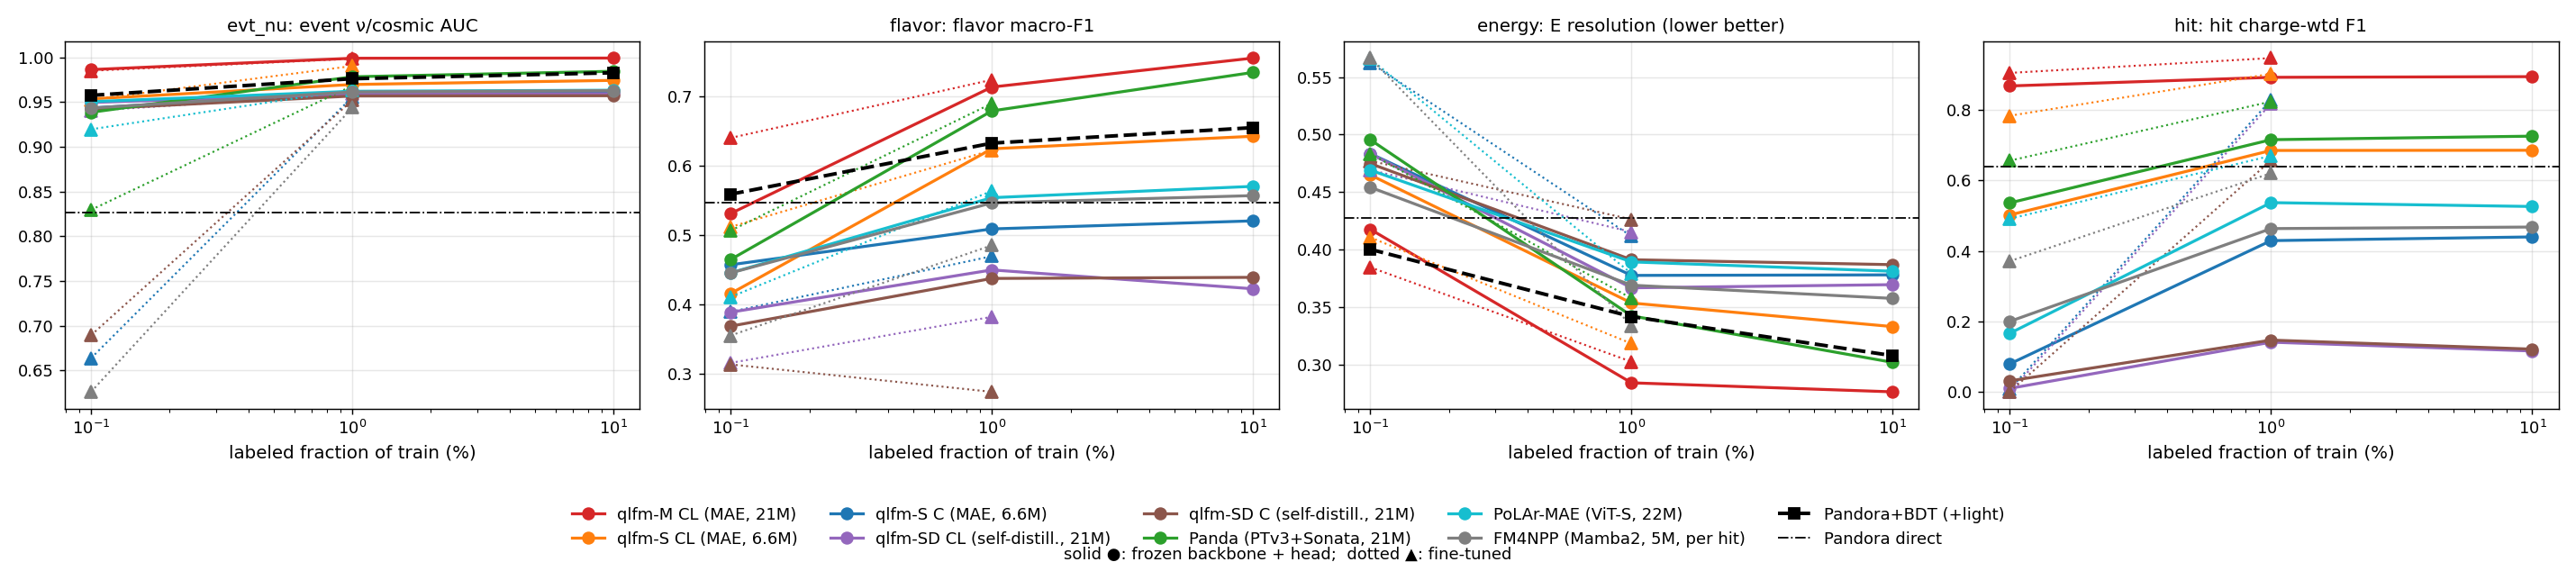
\includegraphics[width=\textwidth]{../figures/round2_comparison.png}
\caption{All four tasks versus label fraction. Solid lines with circles: frozen backbone + head. Dotted lines with triangles: fine-tuned. Black dashed: Pandora+BDT (+light). Dash-dot: Pandora direct.}
\end{figure}

In the tables below, $\pm$ is the spread over 2 seeds; every other entry is a single seed. \pft\ marks the Panda fine-tune entries. They come from a re-run with a trainable backbone; the first runs had trained only the head (Sec.~\ref{sec:caveats}). ``C-only diag'' is the frozen run at 1\% without the late-fused light; qlfm-CL backbones still contain light internally.

\newcommand{\rtabhead}{\toprule
Method & frozen 0.1\% & frozen 1\% & frozen 10\% & FT 0.1\% & FT 1\% & C-only diag\\\midrule}
\begin{table}[H]\centering\small
\caption{T2 event-level $\nu$/cosmic: AUC (in-AV $\nu$ vs no-$\nu$).}
\begin{tabular}{lcccccc}\rtabhead
qlfm-M CL (MAE, 21M) & \best{0.986}$\pm$.002 & \best{0.999} & \best{0.999} & \best{0.985} & \best{0.998} & 0.999\\
qlfm-S CL (MAE, 6.6M) & 0.953$\pm$.001 & 0.970 & 0.974 & 0.953 & 0.990 & 0.972\\
qlfm-S C (MAE, 6.6M) & 0.943$\pm$.001 & 0.960 & 0.962 & 0.664 & 0.956 & 0.666\\
qlfm-SD CL (21M) & 0.949$\pm$.000 & 0.959 & 0.959 & 0.940 & 0.959 & 0.605\\
qlfm-SD C (21M) & 0.942$\pm$.000 & 0.957 & 0.957 & 0.690 & 0.952 & 0.609\\
Panda (21M) & 0.938$\pm$.007 & 0.978 & 0.984 & 0.830\pft & 0.968\pft & 0.914\\
PoLAr-MAE (22M) & 0.950$\pm$.001 & 0.962 & 0.963 & 0.920 & 0.964 & 0.660\\
FM4NPP (4.9M) & 0.943$\pm$.000 & 0.961 & 0.963 & 0.626 & 0.944 & 0.712\\
\midrule
Pandora+BDT C & 0.926$\pm$.001 & 0.949 & 0.955 & & & \\
Pandora+BDT CL & 0.957$\pm$.003 & 0.976 & 0.983 & & & \\
Pandora direct & \multicolumn{3}{c}{0.826 (no training)} & & & \\
\bottomrule\end{tabular}\end{table}

\begin{table}[H]\centering\small
\caption{T3 flavor (\numu CC / \nue CC / NC): macro-F1.}
\begin{tabular}{lcccccc}\rtabhead
qlfm-M CL & 0.531$\pm$.003 & \best{0.713} & \best{0.755} & \best{0.640} & \best{0.724} & 0.709\\
qlfm-S CL & 0.416$\pm$.002 & 0.624 & 0.642 & 0.512 & 0.622 & 0.625\\
qlfm-S C & 0.457$\pm$.000 & 0.509 & 0.520 & 0.389 & 0.469 & 0.429\\
qlfm-SD CL & 0.389$\pm$.003 & 0.450 & 0.423 & 0.316 & 0.382 & 0.297\\
qlfm-SD C & 0.369$\pm$.001 & 0.437 & 0.439 & 0.314 & 0.274 & 0.303\\
Panda & 0.465$\pm$.001 & 0.679 & 0.734 & 0.506\pft & 0.690\pft & 0.666\\
PoLAr-MAE & 0.446$\pm$.004 & 0.554 & 0.570 & 0.411 & 0.563 & 0.497\\
FM4NPP & 0.445$\pm$.003 & 0.546 & 0.557 & 0.355 & 0.485 & 0.507\\
\midrule
Pandora+BDT C & 0.542$\pm$.007 & 0.619 & 0.641 & & & \\
Pandora+BDT CL & \best{0.559}$\pm$.007 & 0.632 & 0.655 & & & \\
Pandora direct & \multicolumn{3}{c}{0.547 (no training)} & & & \\
\bottomrule\end{tabular}\end{table}

\begin{table}[H]\centering\small
\caption{T4 neutrino energy: resolution (lower is better).}
\begin{tabular}{lcccccc}\rtabhead
qlfm-M CL & 0.418$\pm$.003 & \best{0.284} & \best{0.276} & \best{0.385} & \best{0.303} & 0.284\\
qlfm-S CL & 0.465$\pm$.007 & 0.354 & 0.333 & 0.411 & 0.318 & 0.345\\
qlfm-S C & 0.484$\pm$.001 & 0.378 & 0.378 & 0.563 & 0.412 & 0.441\\
qlfm-SD CL & 0.483$\pm$.005 & 0.367 & 0.370 & 0.469 & 0.415 & 0.439\\
qlfm-SD C & 0.475$\pm$.002 & 0.391 & 0.387 & 0.477 & 0.426 & 0.454\\
Panda & 0.496$\pm$.001 & 0.343 & 0.302 & 0.484\pft & 0.358\pft & 0.423\\
PoLAr-MAE & 0.469$\pm$.002 & 0.389 & 0.381 & 0.566 & 0.379 & 0.421\\
FM4NPP & 0.454$\pm$.013 & 0.369 & 0.358 & 0.567 & 0.334 & 0.420\\
\midrule
Pandora+BDT C & 0.407$\pm$.005 & 0.355 & 0.324 & & & \\
Pandora+BDT CL & \best{0.400}$\pm$.005 & 0.342 & 0.308 & & & \\
Pandora direct & \multicolumn{3}{c}{0.428 (calibrated on 100\% of labels)} & & & \\
\bottomrule\end{tabular}\end{table}

\begin{table}[H]\centering\small
\caption{T1 hit-level $\nu$/cosmic: charge-weighted F1. Pandora's $\nu$-slice hits on the same 3k test events: F1$_q$ 0.651 (efficiency 0.784, purity 0.556).}
\begin{tabular}{lcccccc}\rtabhead
qlfm-M CL & \best{0.868}$\pm$.000 & \best{0.892} & \best{0.894} & \best{0.905} & \best{0.947} & 0.891\\
qlfm-S CL & 0.502$\pm$.005 & 0.685 & 0.685 & 0.783 & 0.902 & 0.675\\
qlfm-S C & 0.080$\pm$.001 & 0.429 & 0.440 & 0.008 & 0.828 & 0.170\\
qlfm-SD CL & 0.010$\pm$.001 & 0.141 & 0.116 & 0.001 & 0.818 & 0.000\\
qlfm-SD C & 0.032$\pm$.003 & 0.147 & 0.122 & 0.001 & 0.657 & 0.004\\
Panda & 0.536$\pm$.003 & 0.715 & 0.725 & 0.656\pft & 0.823\pft & 0.629\\
PoLAr-MAE & 0.167$\pm$.025 & 0.537 & 0.526 & 0.491 & 0.670 & 0.351\\
FM4NPP & 0.200$\pm$.013 & 0.463 & 0.468 & 0.371 & 0.620 & 0.238\\
\midrule
Pandora $\nu$ slice & \multicolumn{3}{c}{0.651 (no training)} & & & \\
\bottomrule\end{tabular}\end{table}

%=====================================================================
\section{Event-level analysis and event displays}\label{sec:displays}
%=====================================================================
\subsection{Per-event correctness and selection}
To see \emph{which} events each metric rewards or punishes, we score every test event for 8 algorithms: Pandora direct, Pandora+BDT (+light, 1\% labels, seed 0), and the six foundation models qlfm-M CL, qlfm-S CL, Panda, PoLAr-MAE, FM4NPP and qlfm-SD CL. Each foundation model is frozen with a late-light head at 1\% labels, seed 0.

An algorithm is \emph{correct} on an event if:
\begin{itemize}
  \item T2, T3: its predicted class (argmax) equals the truth;
  \item T4: $|E_\text{pred}/E_\text{true}-1|<0.2$;
  \item T1: its per-event F1$_q\geq0.8$. For T1, ``Pandora'' means its $\nu$-slice hits, and there are 7 algorithms because Pandora+BDT has no hit output.
\end{itemize}

For each task we then select:
\begin{itemize}
  \item \textbf{10 easy events}, those the most algorithms get right;
  \item \textbf{10 boundary events}, where about half the algorithms are correct: 4 of 8 (T1: 3 or 4 of 7), drawn at random. These show what separates the methods;
  \item \textbf{10 hard events}, those the fewest get right.
\end{itemize}
Picks are spread round-robin over truth classes (T4: $E<0.7$, 0.7--1.5, $>1.5$\,GeV). For T1, the hardest events overall all have a $\nu$ charge fraction below 1\%, so 5 hard picks are taken from them and 5 from events with a $\nu$ charge fraction $\geq$5\%.

Fig.~\ref{fig:agree} and Table~\ref{tab:evacc} summarize agreement over the full test subsets.

\begin{figure}[H]\centering
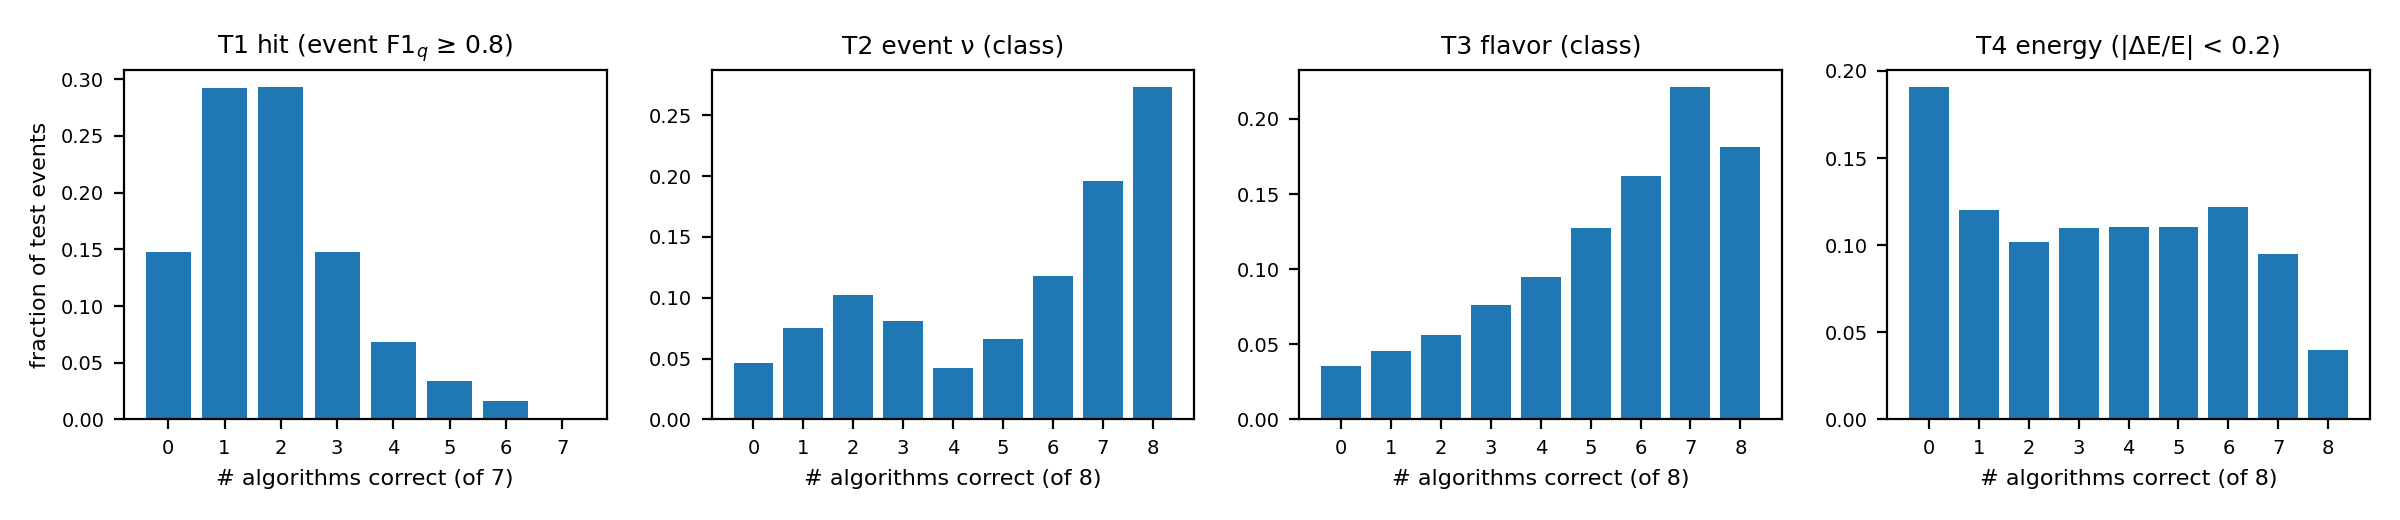
\includegraphics[width=\textwidth]{../figures/round2_agreement.png}
\caption{Distribution of the number of algorithms that are correct on each test event (T1: 3k events, 7 algorithms; T2--T4: 10k events, 8 algorithms).}\label{fig:agree}
\end{figure}

\begin{table}[H]\centering\small
\caption{Per-event accuracy under the correctness rules above (T2: 3-class accuracy, including out-of-AV). ``Hard'': accuracy on the consensus-hard events, those where $\leq$1 algorithm is correct (T1: none correct). Their counts are 1{,}208 (T2), 810 (T3), 3{,}106 (T4) and 444 (T1).}\label{tab:evacc}
\begin{tabular}{lcccccccc}
\toprule
& \multicolumn{2}{c}{T1 hit} & \multicolumn{2}{c}{T2 event $\nu$} & \multicolumn{2}{c}{T3 flavor} & \multicolumn{2}{c}{T4 energy}\\
Algorithm & all & hard & all & hard & all & hard & all & hard\\
\midrule
qlfm-M CL & \best{0.786} & 0 & \best{0.755} & \best{0.242} & \best{0.800} & 0.081 & \best{0.485} & \best{0.094}\\
qlfm-S CL & 0.212 & 0 & 0.677 & 0.030 & 0.710 & 0.033 & 0.430 & 0.054\\
Panda & 0.249 & 0 & 0.727 & 0.136 & 0.742 & \best{0.179} & 0.434 & 0.082\\
PoLAr-MAE & 0.066 & 0 & 0.668 & 0.006 & 0.638 & 0.022 & 0.403 & 0.008\\
FM4NPP & 0.043 & 0 & 0.666 & 0.006 & 0.640 & 0.037 & 0.390 & 0.011\\
qlfm-SD CL & 0.000 & 0 & 0.666 & 0.010 & 0.537 & 0.054 & 0.389 & 0.008\\
Pandora direct / $\nu$ slice & 0.509 & 0 & 0.437 & 0.096 & 0.593 & 0.093 & 0.383 & 0.052\\
Pandora+BDT (+light) & -- & -- & 0.692 & 0.094 & 0.712 & 0.060 & 0.451 & 0.076\\
\bottomrule
\end{tabular}
\end{table}

\subsection{What the hard events have in common}
\begin{description}[leftmargin=1.2em]
\item[T2.] Of the 1{,}208 consensus-hard events, 832 are out-of-AV $\nu$ (class 2), although that class is 34\% of the test set. The foundation-model majority calls them no-$\nu$ (426) or in-AV $\nu$ (406). The reverse confusions, in-AV called out-of-AV (215) and no-$\nu$ called out-of-AV (108), are the next largest.

  The class-0/2 boundary ($\leq$5 vs $>$5 $\nu$ hits) and the class-1/2 boundary (vertex inside the AV with $\geq$30 collection hits) are sharp in truth but nearly invisible in the data. Display T2-hard~\#1 is an example: a \numu CC with its vertex 10\,cm below the AV leaves at most 5 $\nu$ hits next to a beam-coincident flash. It is labelled no-$\nu$, while every foundation model and the BDT call it out-of-AV $\nu$.

  The headline AUC (class 1 vs 0) avoids class 2 entirely, which is why it is near 1 while the 3-class accuracy is 0.67--0.76.
\item[T3.] The consensus-hard events are evenly split by truth: 211 \numu CC, 283 \nue CC and 316 NC. The dominant confusions are NC $\to$ \numu CC (257), \nue CC $\to$ \numu CC (186) and \numu CC $\to$ NC (151). These are the expected physics ambiguities: a short or absent muon track, $\pi^0$ showers, and electrons hidden under cosmics. Panda is the best on this hard subset (0.18), suggesting its point-level features keep finer topology than cell tokens.
\item[T4.] Consensus-hard events sit in the tails: the median $E_\nu$ is 1.31\,GeV versus 1.14 overall, and the 10--90\% range is 0.47--2.99\,GeV versus 0.63--2.10. All regressors shrink toward the mean, so low-energy events are over-predicted and high-energy events under-predicted. The foundation-model mean is too high for 45\% of these events.
\item[T1.] No event is correct for all 7 algorithms, because qlfm-SD never reaches F1$_q\geq0.8$ on any event. The 444 events that every algorithm misses have a median $\nu$ charge fraction of 2.6\%, against 5.6\% overall. A small $\nu$ (a few short tracks next to tens of cosmics) is the main failure mode for every method, Pandora included.

  On typical events qlfm-M is clearly ahead. Its per-event median F1$_q$ is 0.91, against 0.81 for Pandora's $\nu$ slice and 0.67, 0.64, 0.42, 0.32 and 0.01 for Panda, qlfm-S, PoLAr-MAE, FM4NPP and qlfm-SD.
\end{description}

\subsection{What separates the methods: boundary events}
Boundary events are those where exactly half of the algorithms are correct (T1: 3 or 4 of 7). Table~\ref{tab:bnd} gives each algorithm's accuracy on all such test events. By construction the average is about 50\%; the spread shows who wins the split cases.
\begin{table}[H]\centering\small
\caption{Per-algorithm accuracy on boundary test events. The number of such events is in parentheses.}\label{tab:bnd}
\begin{tabular}{lcccc}
\toprule
Algorithm & T1 hit (650) & T2 event $\nu$ (421) & T3 flavor (949) & T4 energy (1{,}104)\\
\midrule
qlfm-M CL & \best{0.998} & 0.577 & \best{0.737} & \best{0.618}\\
qlfm-S CL & 0.617 & 0.568 & 0.537 & 0.533\\
Panda & 0.672 & \best{0.587} & 0.640 & 0.528\\
PoLAr-MAE & 0.102 & 0.442 & 0.380 & 0.443\\
FM4NPP & 0.054 & 0.542 & 0.401 & 0.432\\
qlfm-SD CL & 0.000 & 0.508 & 0.359 & 0.446\\
Pandora direct / $\nu$ slice & 0.874 & 0.240 & 0.399 & 0.459\\
Pandora+BDT (+light) & -- & 0.537 & 0.546 & 0.542\\
\bottomrule
\end{tabular}
\end{table}
\begin{itemize}
  \item \textbf{T1:} on the split events, the winners are almost always qlfm-M (99.8\%) and Pandora's $\nu$ slice (87\%), followed by Panda and qlfm-S.
  \item \textbf{T3:} qlfm-M is right on 74\% of split events, against 64\% for Panda and 55\% for the BDT.
  \item \textbf{T4:} qlfm-M is right on 62\% of split events; the others are at 43--54\%.
  \item \textbf{T2:} the split is nearly even among the light-using models (54--59\%); Pandora direct cannot predict the out-of-AV class and is lowest.
\end{itemize}

\subsection{Selected examples}
These are referred to by their appendix labels.
\begin{description}[leftmargin=1.2em]
\item[T1 easy \#1] A 1.6\,GeV \nue CC shower downstream (vertex $z=910$\,cm), carrying 16\% of the event charge. The flash is centred on the vertex. Six of the seven algorithms reach F1$_q\geq0.94$. qlfm-SD (0.77) also tags parts of nearby cosmics, the diffuse $p(\nu)$ typical of its weak per-hit features.
\item[T1 hard \#7] A 1.6\,GeV \numu CC with its vertex near the top of the TPC ($y=111$\,cm), crossed by several cosmics. Pandora's $\nu$ slice is a neighbouring cosmic track (F1$_q=0$). qlfm-M recovers about half of the $\nu$ charge (0.45) and Panda about a third (0.30). qlfm-S reaches 0.16; PoLAr-MAE, FM4NPP and qlfm-SD find nothing.
\item[T2 hard \#1] Discussed above. A \numu CC with its vertex just below the AV is labelled no-$\nu$. The flash matched to the true interaction time sits directly above the vertex ($z\approx500$\,cm, bottom PMTs), so the $\nu$'s light is in the event even though it left at most 5 hits. Every foundation model therefore says ``out-of-AV $\nu$''. This is a label-boundary case, not a detector-level failure.
\item[T3 boundary \#2] A 2.8\,GeV \nue CC with a long, track-like secondary next to the electron shower. The algorithms split 4--4 between \nue CC and \numu CC (Panda says NC).
  \begin{itemize}
    \item qlfm-M separates the $\nu$ hits almost perfectly (F1$_q=0.98$) but calls the event \numu CC.
    \item The smaller qlfm-S, PoLAr-MAE, FM4NPP and the BDT get it right.
  \end{itemize}
  A typical boundary case: a long track makes the event look \numu-like.
\item[T3 hard \#1] A 0.5\,GeV \numu CC with its vertex 15\,cm below the top of the AV. Only a few short $\nu$ tracks are visible, and all eight algorithms call it NC. Without a clearly identifiable muon, low-energy \numu CC is topologically NC-like.
\item[T4 hard \#4] A 0.35\,GeV \numu CC at $z=142$\,cm lies next to a large, bright cosmic-induced deposit at the same drift time, and the beam flash covers both.
  \begin{itemize}
    \item Pandora's $\nu$ slice absorbs that deposit, giving $E=1.87$\,GeV ($+429$\%).
    \item Every foundation model overestimates too, by $+81$\% to $+154$\%.
    \item qlfm-M's hit head isolates the $\nu$ hits well (F1$_q=0.86$), but its energy head is a separate attentive pool over all tokens and does not use that separation.
  \end{itemize}
  This suggests a task-coupled head that conditions energy on the predicted $\nu$ hits.
\end{description}

\subsection{How to read the displays}
Appendix~\ref{app:displays} shows all 120 selected events, one per page. Each page contains:
\begin{itemize}
  \item a header with the task, easy or hard, the number of correct algorithms, run/subrun/event, the truth ($\nu$ flavor, CC/NC, energy, vertex, task label) and each algorithm's task prediction (\checkmark\ / $\times$);
  \item \textbf{Charge}: every hit at (global channel, tick), coloured by $\log_{10}$ integral. U, V and Y are concatenated (channels 0--2399, 2400--4799, 4800--8255). Tick increases downward, i.e.\ away from the anode;
  \item \textbf{PMT view} (inspired by BEE): each PMT drawn at its $(z,y)$ position. Circle area is proportional to that PMT's PE (scaled to the brightest PMT of the event) in the optical flash \emph{belonging to the $\nu$ interaction}. Grey rings mark all 32 PMTs; the star marks the true $\nu$ vertex.
  \begin{itemize}
    \item The open data store the true interaction time $t_\nu$ (in \code{event\_table/nu\_vtx\_wire\_time}, ns, spanning the 1.6\,$\mu$s BNB spill). The reconstructed flash time lags it by $0.478\,\mu$s: median over visible-$\nu$ events, 5--95\% range 0.457--0.506\,$\mu$s.
    \item From all flashes of the event (\code{opflash\_table}, \code{opflashsumpe\_table}) we show the one closest to $t_\nu+0.478\,\mu$s, if it lies within 1\,$\mu$s.
    \item Without a truth time the fallback would be the flash closest to the typical beam-flash time (4.56\,$\mu$s), not $t=0$. In these files the beam flashes sit at about 3.6--5.2\,$\mu$s after the time reference, and cosmic flashes occur throughout the readout window. Every overlay event carries a truth time, so the fallback is never used here.
    \item The panel title gives the flash time, its PE, the number of flashes, and whether the matched flash is also the largest. For 4.5\% of visible-$\nu$ events with a flash, the largest flash is more than 0.3\,$\mu$s from the expected $\nu$ flash time, i.e.\ it is not the $\nu$ flash. Among the 120 displayed events, 6 have a matched flash that is not the largest, and 13 have no reconstructed flash within 1\,$\mu$s. In those 13 the panel instead sums the optical hits within $[-0.5,+3.5]\,\mu$s of the expected time.
    \begin{itemize}
      \item 10 of the 13 are out-of-AV $\nu$ with at most 16 $\nu$ hits, so there is little or no light.
      \item 3 are in-AV $\nu$ whose event has no beam-time flash in \code{opflash\_table}: the only flashes are at $-59$ and 3404\,$\mu$s, and one is 1.1\,$\mu$s early.
    \end{itemize}
  \end{itemize}
  \item \textbf{eight hit panels}: Truth ($\nu$ = red), Pandora ($\nu$-slice hits), and the six foundation-model hit heads (frozen, 1\%, late light). Colour is $p(\nu)$ from blue (cosmic) to red ($\nu$). Each title gives that algorithm's per-event F1$_q$. Dashed boxes mark the 1--99\% extent of the true $\nu$ hits in each plane.
\end{itemize}
The hit panels are shown for every event, not only the T1 selection, so the event-level predictions can be compared with how each backbone separates $\nu$ from cosmic charge in the same event. The hit probabilities come from re-running the frozen 1\% T1 heads on these 120 events (batch 4 instead of 32, bf16). The per-event F1$_q$ agrees with the original test predictions to within 0.01 for the qlfm models and FM4NPP, 0.03 for PoLAr-MAE and 0.06 for Panda.

%=====================================================================
\section{Discussion}
%=====================================================================
\begin{itemize}[leftmargin=*]
\item \textbf{Versus the open-data reconstruction.}
  \begin{itemize}
    \item Every foundation model with light beats Pandora's direct \code{nu\_score} on T2 by a wide margin (0.94--0.999 vs 0.83).
    \item On per-hit T1, only qlfm-M (all modes), qlfm-S CL (fine-tuned) and Panda (frozen at $\geq$1\% labels; fine-tuned: 0.656 and 0.823) beat Pandora's $\nu$ slice.
    \item Pandora+BDT is the tougher reference. Its 40 reconstruction features are very label-efficient but saturate early.
    \item The BDT's own gain from light (+0.02--0.03 AUC on T2) shows light still carries information after reconstruction.
  \end{itemize}
\item \textbf{Versus other foundation-model recipes at equal compute.}
  \begin{itemize}
    \item At matched size (about 21M) and node-hours, qlfm-M's multi-modal MAE with early light fusion gives the best frozen features on every task.
    \item Panda is the clear runner-up and the best charge-only representation.
    \item There is no charge-only qlfm model at 21M, so how much of qlfm-M's edge comes from early fusion versus the MAE objective versus the cell tokenizer is still open.
  \end{itemize}
\item \textbf{FM4NPP and PoLAr-MAE} learn useful but weaker features under these adaptations.
  \begin{itemize}
    \item FM4NPP: plausible limits are causal per-hit serialization of cosmic-dominated 2D projections, the relative-offset objective, and its small (4.9M) size.
    \item PoLAr-MAE: plausible limits are coarse 4\,cm groups along long cosmic tracks.
  \end{itemize}
\item \textbf{qlfm-SD} gives poor per-hit and mediocre event features at this budget. Likely causes are the low learning rate, the drift-window crops, and dropping masked tokens without a mask token. A tuned qlfm-SD is a candidate for round~3.
\item \textbf{Fine-tuning at 0.1\% labels} (a few hundred events) is unstable for several backbones, e.g.\ FM4NPP T2 0.63, qlfm-S C 0.66 and Panda 0.83. Frozen probes are the more reliable low-label mode.
\end{itemize}

%=====================================================================
\section{Limitations and caveats}\label{sec:caveats}
%=====================================================================
\begin{itemize}[leftmargin=*]
\item \textbf{Panda fine-tune was re-run (\pft).} The downstream Panda backbone is the \code{pimm} Sonata teacher, whose parameters \code{pimm} sets to \code{requires\_grad=False}.
  \begin{itemize}
    \item The first fine-tune runs therefore trained only the 2.30M head parameters.
    \item The backbone is now explicitly made trainable (20.6M + head). All 8 runs were repeated with the same protocol and gradient accumulation $8\times4$; all reached the full step count.
    \item The tables show the re-run. The head-only results were 0.937/0.974 (T2), 0.492/0.642 (T3), 0.476/0.341 (T4) and 0.381/0.653 (T1) at 0.1\%/1\%.
    \item True fine-tuning helps Panda most on hits (T1 0.656/0.823 vs frozen 0.536/0.715) and on flavor at 1\% (0.690 vs 0.679). Like the other backbones, it is unstable for T2 at 0.1\% (0.830).
  \end{itemize}
\item \textbf{PoLAr-MAE fine-tuning} also counts the MAE decoder as trainable. The decoder gets no gradient, so this inflates only the parameter count. Encoder drop-path (0.25) is active during fine-tuning.
\item \textbf{Five runs hit the time limit before 3{,}000 steps}: FM4NPP T1 FT 1\% (1{,}800 steps), FM4NPP T1 C-only (1{,}500), and PoLAr-MAE FT 1\% on T1, T2 and T3 (2{,}400--2{,}700). Fine-tuned heavy backbones may be under-trained in general.
\item \textbf{Gradient accumulation} ($4\times8$) was used where memory required it. The optimizer batch is always 32.
\item \textbf{Pandora test subsets.} The Pandora references are scored on a 20k-event test subset, a superset of the neural 10k subset drawn from the same permutation. The Pandora-direct energy calibration uses all training labels.
\item \textbf{Scope of the comparison.} Every reference is an \emph{adaptation} (2D planes, sizes, targets) trained for about 4 node-hours, far less than its published schedule; Panda, for example, saw about 18\% of its published samples. The results compare these adaptations at equal compute, not the published models.
\item \textbf{Statistics and data.} Most entries are single-seed; differences below about 0.02 are not significant. Pandora+BDT uses only the HDF5-level reconstruction. Round~1's overlay-only caveats apply.
\end{itemize}

%=====================================================================
\section{Reproducibility and compute}
%=====================================================================
\sloppy
\begin{itemize}[leftmargin=*]
\item Pandora references: \code{python -m qlfm.data.pandora\_features}, \code{scripts/pandora\_refs.py}. Per-event predictions: \code{scripts/pandora\_event\_preds.py}.
\item Pretraining:
  \begin{itemize}
    \item \code{qlfm.train\_pretrain} with \code{--method \{mae,sd,fm4npp\}}; FM4NPP runs in the \code{mamba\_ssm} venv.
    \item Panda and PoLAr-MAE: \code{qlfm/ref/pimm\_train.py} with the configs in \code{qlfm/ref/pimm\_configs/}, in the pimm venv.
  \end{itemize}
\item Downstream: \code{scripts/make\_tasks\_r2.py}, then \code{scripts/run\_queue.sh}. Tables: \code{scripts/summarize\_r2.py}.
\item Event displays:
  \begin{itemize}
    \item \code{scripts/r2\_select\_events.py} (selection) and \code{scripts/r2\_agreement.py} (statistics);
    \item \code{scripts/infer\_hits.py} via \code{scripts/pbs/infer\_hits.pbs} (per-hit inference);
    \item \code{scripts/r2\_event\_displays.py} (rendering).
  \end{itemize}
\item Compute: 37.6 node-hours for the comparison, plus 1.1 for the display inference and the Panda fine-tune re-run, 38.7 in total (\code{docs/figures/round2\_node\_hours.md}).
\end{itemize}

\begin{thebibliography}{99}\small
\bibitem{ubopendata} G.~Cerati (for MicroBooNE), \emph{MicroBooNE public data sets: a collaborative tool for LArTPC software development}, arXiv:2309.15362.
\bibitem{polarmae} \emph{Particle trajectory representation learning with masked point modeling} (PoLAr-MAE), arXiv:2502.02558.
\bibitem{fm4npp} \emph{FM4NPP: a scaling foundation model for nuclear and particle physics}, arXiv:2508.14087.
\bibitem{panda} \emph{Panda: self-distillation of reusable sensor-level representations for high energy physics}, arXiv:2512.01324.
\bibitem{pandav2} \emph{Panda Diplomacy: foundation model pre-training across particle imaging detectors}, arXiv:2609.00611.
\bibitem{sonata} X.~Wu et al., \emph{Sonata: self-supervised learning of reliable point representations}, arXiv:2503.16429.
\end{thebibliography}

\clearpage
\appendix
\newgeometry{margin=0.8cm,bottom=1.2cm}
\section{Event displays}\label{app:displays}
One page per selected event: for each task, 10 easy events (most algorithms correct), then 10 boundary events (about half correct), then 10 hard events (fewest correct). The selection rules are in Sec.~\ref{sec:displays}. Hit panels use the frozen 1\% T1 heads of every foundation model, regardless of the task the event was selected for.
\subsection{T1: hit-level $\nu$/cosmic}
\begin{center}\includegraphics[height=0.86\textheight,width=\textwidth,keepaspectratio]{displays/hit_easy01.png}\end{center}\clearpage
\begin{center}\includegraphics[height=0.86\textheight,width=\textwidth,keepaspectratio]{displays/hit_easy02.png}\end{center}\clearpage
\begin{center}\includegraphics[height=0.86\textheight,width=\textwidth,keepaspectratio]{displays/hit_easy03.png}\end{center}\clearpage
\begin{center}\includegraphics[height=0.86\textheight,width=\textwidth,keepaspectratio]{displays/hit_easy04.png}\end{center}\clearpage
\begin{center}\includegraphics[height=0.86\textheight,width=\textwidth,keepaspectratio]{displays/hit_easy05.png}\end{center}\clearpage
\begin{center}\includegraphics[height=0.86\textheight,width=\textwidth,keepaspectratio]{displays/hit_easy06.png}\end{center}\clearpage
\begin{center}\includegraphics[height=0.86\textheight,width=\textwidth,keepaspectratio]{displays/hit_easy07.png}\end{center}\clearpage
\begin{center}\includegraphics[height=0.86\textheight,width=\textwidth,keepaspectratio]{displays/hit_easy08.png}\end{center}\clearpage
\begin{center}\includegraphics[height=0.86\textheight,width=\textwidth,keepaspectratio]{displays/hit_easy09.png}\end{center}\clearpage
\begin{center}\includegraphics[height=0.86\textheight,width=\textwidth,keepaspectratio]{displays/hit_easy10.png}\end{center}\clearpage
\begin{center}\includegraphics[height=0.86\textheight,width=\textwidth,keepaspectratio]{displays/hit_boundary01.png}\end{center}\clearpage
\begin{center}\includegraphics[height=0.86\textheight,width=\textwidth,keepaspectratio]{displays/hit_boundary02.png}\end{center}\clearpage
\begin{center}\includegraphics[height=0.86\textheight,width=\textwidth,keepaspectratio]{displays/hit_boundary03.png}\end{center}\clearpage
\begin{center}\includegraphics[height=0.86\textheight,width=\textwidth,keepaspectratio]{displays/hit_boundary04.png}\end{center}\clearpage
\begin{center}\includegraphics[height=0.86\textheight,width=\textwidth,keepaspectratio]{displays/hit_boundary05.png}\end{center}\clearpage
\begin{center}\includegraphics[height=0.86\textheight,width=\textwidth,keepaspectratio]{displays/hit_boundary06.png}\end{center}\clearpage
\begin{center}\includegraphics[height=0.86\textheight,width=\textwidth,keepaspectratio]{displays/hit_boundary07.png}\end{center}\clearpage
\begin{center}\includegraphics[height=0.86\textheight,width=\textwidth,keepaspectratio]{displays/hit_boundary08.png}\end{center}\clearpage
\begin{center}\includegraphics[height=0.86\textheight,width=\textwidth,keepaspectratio]{displays/hit_boundary09.png}\end{center}\clearpage
\begin{center}\includegraphics[height=0.86\textheight,width=\textwidth,keepaspectratio]{displays/hit_boundary10.png}\end{center}\clearpage
\begin{center}\includegraphics[height=0.86\textheight,width=\textwidth,keepaspectratio]{displays/hit_hard01.png}\end{center}\clearpage
\begin{center}\includegraphics[height=0.86\textheight,width=\textwidth,keepaspectratio]{displays/hit_hard02.png}\end{center}\clearpage
\begin{center}\includegraphics[height=0.86\textheight,width=\textwidth,keepaspectratio]{displays/hit_hard03.png}\end{center}\clearpage
\begin{center}\includegraphics[height=0.86\textheight,width=\textwidth,keepaspectratio]{displays/hit_hard04.png}\end{center}\clearpage
\begin{center}\includegraphics[height=0.86\textheight,width=\textwidth,keepaspectratio]{displays/hit_hard05.png}\end{center}\clearpage
\begin{center}\includegraphics[height=0.86\textheight,width=\textwidth,keepaspectratio]{displays/hit_hard06.png}\end{center}\clearpage
\begin{center}\includegraphics[height=0.86\textheight,width=\textwidth,keepaspectratio]{displays/hit_hard07.png}\end{center}\clearpage
\begin{center}\includegraphics[height=0.86\textheight,width=\textwidth,keepaspectratio]{displays/hit_hard08.png}\end{center}\clearpage
\begin{center}\includegraphics[height=0.86\textheight,width=\textwidth,keepaspectratio]{displays/hit_hard09.png}\end{center}\clearpage
\begin{center}\includegraphics[height=0.86\textheight,width=\textwidth,keepaspectratio]{displays/hit_hard10.png}\end{center}\clearpage
\clearpage\subsection{T2: event-level $\nu$ presence}
\begin{center}\includegraphics[height=0.86\textheight,width=\textwidth,keepaspectratio]{displays/evt_nu_easy01.png}\end{center}\clearpage
\begin{center}\includegraphics[height=0.86\textheight,width=\textwidth,keepaspectratio]{displays/evt_nu_easy02.png}\end{center}\clearpage
\begin{center}\includegraphics[height=0.86\textheight,width=\textwidth,keepaspectratio]{displays/evt_nu_easy03.png}\end{center}\clearpage
\begin{center}\includegraphics[height=0.86\textheight,width=\textwidth,keepaspectratio]{displays/evt_nu_easy04.png}\end{center}\clearpage
\begin{center}\includegraphics[height=0.86\textheight,width=\textwidth,keepaspectratio]{displays/evt_nu_easy05.png}\end{center}\clearpage
\begin{center}\includegraphics[height=0.86\textheight,width=\textwidth,keepaspectratio]{displays/evt_nu_easy06.png}\end{center}\clearpage
\begin{center}\includegraphics[height=0.86\textheight,width=\textwidth,keepaspectratio]{displays/evt_nu_easy07.png}\end{center}\clearpage
\begin{center}\includegraphics[height=0.86\textheight,width=\textwidth,keepaspectratio]{displays/evt_nu_easy08.png}\end{center}\clearpage
\begin{center}\includegraphics[height=0.86\textheight,width=\textwidth,keepaspectratio]{displays/evt_nu_easy09.png}\end{center}\clearpage
\begin{center}\includegraphics[height=0.86\textheight,width=\textwidth,keepaspectratio]{displays/evt_nu_easy10.png}\end{center}\clearpage
\begin{center}\includegraphics[height=0.86\textheight,width=\textwidth,keepaspectratio]{displays/evt_nu_boundary01.png}\end{center}\clearpage
\begin{center}\includegraphics[height=0.86\textheight,width=\textwidth,keepaspectratio]{displays/evt_nu_boundary02.png}\end{center}\clearpage
\begin{center}\includegraphics[height=0.86\textheight,width=\textwidth,keepaspectratio]{displays/evt_nu_boundary03.png}\end{center}\clearpage
\begin{center}\includegraphics[height=0.86\textheight,width=\textwidth,keepaspectratio]{displays/evt_nu_boundary04.png}\end{center}\clearpage
\begin{center}\includegraphics[height=0.86\textheight,width=\textwidth,keepaspectratio]{displays/evt_nu_boundary05.png}\end{center}\clearpage
\begin{center}\includegraphics[height=0.86\textheight,width=\textwidth,keepaspectratio]{displays/evt_nu_boundary06.png}\end{center}\clearpage
\begin{center}\includegraphics[height=0.86\textheight,width=\textwidth,keepaspectratio]{displays/evt_nu_boundary07.png}\end{center}\clearpage
\begin{center}\includegraphics[height=0.86\textheight,width=\textwidth,keepaspectratio]{displays/evt_nu_boundary08.png}\end{center}\clearpage
\begin{center}\includegraphics[height=0.86\textheight,width=\textwidth,keepaspectratio]{displays/evt_nu_boundary09.png}\end{center}\clearpage
\begin{center}\includegraphics[height=0.86\textheight,width=\textwidth,keepaspectratio]{displays/evt_nu_boundary10.png}\end{center}\clearpage
\begin{center}\includegraphics[height=0.86\textheight,width=\textwidth,keepaspectratio]{displays/evt_nu_hard01.png}\end{center}\clearpage
\begin{center}\includegraphics[height=0.86\textheight,width=\textwidth,keepaspectratio]{displays/evt_nu_hard02.png}\end{center}\clearpage
\begin{center}\includegraphics[height=0.86\textheight,width=\textwidth,keepaspectratio]{displays/evt_nu_hard03.png}\end{center}\clearpage
\begin{center}\includegraphics[height=0.86\textheight,width=\textwidth,keepaspectratio]{displays/evt_nu_hard04.png}\end{center}\clearpage
\begin{center}\includegraphics[height=0.86\textheight,width=\textwidth,keepaspectratio]{displays/evt_nu_hard05.png}\end{center}\clearpage
\begin{center}\includegraphics[height=0.86\textheight,width=\textwidth,keepaspectratio]{displays/evt_nu_hard06.png}\end{center}\clearpage
\begin{center}\includegraphics[height=0.86\textheight,width=\textwidth,keepaspectratio]{displays/evt_nu_hard07.png}\end{center}\clearpage
\begin{center}\includegraphics[height=0.86\textheight,width=\textwidth,keepaspectratio]{displays/evt_nu_hard08.png}\end{center}\clearpage
\begin{center}\includegraphics[height=0.86\textheight,width=\textwidth,keepaspectratio]{displays/evt_nu_hard09.png}\end{center}\clearpage
\begin{center}\includegraphics[height=0.86\textheight,width=\textwidth,keepaspectratio]{displays/evt_nu_hard10.png}\end{center}\clearpage
\clearpage\subsection{T3: flavor}
\begin{center}\includegraphics[height=0.86\textheight,width=\textwidth,keepaspectratio]{displays/flavor_easy01.png}\end{center}\clearpage
\begin{center}\includegraphics[height=0.86\textheight,width=\textwidth,keepaspectratio]{displays/flavor_easy02.png}\end{center}\clearpage
\begin{center}\includegraphics[height=0.86\textheight,width=\textwidth,keepaspectratio]{displays/flavor_easy03.png}\end{center}\clearpage
\begin{center}\includegraphics[height=0.86\textheight,width=\textwidth,keepaspectratio]{displays/flavor_easy04.png}\end{center}\clearpage
\begin{center}\includegraphics[height=0.86\textheight,width=\textwidth,keepaspectratio]{displays/flavor_easy05.png}\end{center}\clearpage
\begin{center}\includegraphics[height=0.86\textheight,width=\textwidth,keepaspectratio]{displays/flavor_easy06.png}\end{center}\clearpage
\begin{center}\includegraphics[height=0.86\textheight,width=\textwidth,keepaspectratio]{displays/flavor_easy07.png}\end{center}\clearpage
\begin{center}\includegraphics[height=0.86\textheight,width=\textwidth,keepaspectratio]{displays/flavor_easy08.png}\end{center}\clearpage
\begin{center}\includegraphics[height=0.86\textheight,width=\textwidth,keepaspectratio]{displays/flavor_easy09.png}\end{center}\clearpage
\begin{center}\includegraphics[height=0.86\textheight,width=\textwidth,keepaspectratio]{displays/flavor_easy10.png}\end{center}\clearpage
\begin{center}\includegraphics[height=0.86\textheight,width=\textwidth,keepaspectratio]{displays/flavor_boundary01.png}\end{center}\clearpage
\begin{center}\includegraphics[height=0.86\textheight,width=\textwidth,keepaspectratio]{displays/flavor_boundary02.png}\end{center}\clearpage
\begin{center}\includegraphics[height=0.86\textheight,width=\textwidth,keepaspectratio]{displays/flavor_boundary03.png}\end{center}\clearpage
\begin{center}\includegraphics[height=0.86\textheight,width=\textwidth,keepaspectratio]{displays/flavor_boundary04.png}\end{center}\clearpage
\begin{center}\includegraphics[height=0.86\textheight,width=\textwidth,keepaspectratio]{displays/flavor_boundary05.png}\end{center}\clearpage
\begin{center}\includegraphics[height=0.86\textheight,width=\textwidth,keepaspectratio]{displays/flavor_boundary06.png}\end{center}\clearpage
\begin{center}\includegraphics[height=0.86\textheight,width=\textwidth,keepaspectratio]{displays/flavor_boundary07.png}\end{center}\clearpage
\begin{center}\includegraphics[height=0.86\textheight,width=\textwidth,keepaspectratio]{displays/flavor_boundary08.png}\end{center}\clearpage
\begin{center}\includegraphics[height=0.86\textheight,width=\textwidth,keepaspectratio]{displays/flavor_boundary09.png}\end{center}\clearpage
\begin{center}\includegraphics[height=0.86\textheight,width=\textwidth,keepaspectratio]{displays/flavor_boundary10.png}\end{center}\clearpage
\begin{center}\includegraphics[height=0.86\textheight,width=\textwidth,keepaspectratio]{displays/flavor_hard01.png}\end{center}\clearpage
\begin{center}\includegraphics[height=0.86\textheight,width=\textwidth,keepaspectratio]{displays/flavor_hard02.png}\end{center}\clearpage
\begin{center}\includegraphics[height=0.86\textheight,width=\textwidth,keepaspectratio]{displays/flavor_hard03.png}\end{center}\clearpage
\begin{center}\includegraphics[height=0.86\textheight,width=\textwidth,keepaspectratio]{displays/flavor_hard04.png}\end{center}\clearpage
\begin{center}\includegraphics[height=0.86\textheight,width=\textwidth,keepaspectratio]{displays/flavor_hard05.png}\end{center}\clearpage
\begin{center}\includegraphics[height=0.86\textheight,width=\textwidth,keepaspectratio]{displays/flavor_hard06.png}\end{center}\clearpage
\begin{center}\includegraphics[height=0.86\textheight,width=\textwidth,keepaspectratio]{displays/flavor_hard07.png}\end{center}\clearpage
\begin{center}\includegraphics[height=0.86\textheight,width=\textwidth,keepaspectratio]{displays/flavor_hard08.png}\end{center}\clearpage
\begin{center}\includegraphics[height=0.86\textheight,width=\textwidth,keepaspectratio]{displays/flavor_hard09.png}\end{center}\clearpage
\begin{center}\includegraphics[height=0.86\textheight,width=\textwidth,keepaspectratio]{displays/flavor_hard10.png}\end{center}\clearpage
\clearpage\subsection{T4: neutrino energy}
\begin{center}\includegraphics[height=0.86\textheight,width=\textwidth,keepaspectratio]{displays/energy_easy01.png}\end{center}\clearpage
\begin{center}\includegraphics[height=0.86\textheight,width=\textwidth,keepaspectratio]{displays/energy_easy02.png}\end{center}\clearpage
\begin{center}\includegraphics[height=0.86\textheight,width=\textwidth,keepaspectratio]{displays/energy_easy03.png}\end{center}\clearpage
\begin{center}\includegraphics[height=0.86\textheight,width=\textwidth,keepaspectratio]{displays/energy_easy04.png}\end{center}\clearpage
\begin{center}\includegraphics[height=0.86\textheight,width=\textwidth,keepaspectratio]{displays/energy_easy05.png}\end{center}\clearpage
\begin{center}\includegraphics[height=0.86\textheight,width=\textwidth,keepaspectratio]{displays/energy_easy06.png}\end{center}\clearpage
\begin{center}\includegraphics[height=0.86\textheight,width=\textwidth,keepaspectratio]{displays/energy_easy07.png}\end{center}\clearpage
\begin{center}\includegraphics[height=0.86\textheight,width=\textwidth,keepaspectratio]{displays/energy_easy08.png}\end{center}\clearpage
\begin{center}\includegraphics[height=0.86\textheight,width=\textwidth,keepaspectratio]{displays/energy_easy09.png}\end{center}\clearpage
\begin{center}\includegraphics[height=0.86\textheight,width=\textwidth,keepaspectratio]{displays/energy_easy10.png}\end{center}\clearpage
\begin{center}\includegraphics[height=0.86\textheight,width=\textwidth,keepaspectratio]{displays/energy_boundary01.png}\end{center}\clearpage
\begin{center}\includegraphics[height=0.86\textheight,width=\textwidth,keepaspectratio]{displays/energy_boundary02.png}\end{center}\clearpage
\begin{center}\includegraphics[height=0.86\textheight,width=\textwidth,keepaspectratio]{displays/energy_boundary03.png}\end{center}\clearpage
\begin{center}\includegraphics[height=0.86\textheight,width=\textwidth,keepaspectratio]{displays/energy_boundary04.png}\end{center}\clearpage
\begin{center}\includegraphics[height=0.86\textheight,width=\textwidth,keepaspectratio]{displays/energy_boundary05.png}\end{center}\clearpage
\begin{center}\includegraphics[height=0.86\textheight,width=\textwidth,keepaspectratio]{displays/energy_boundary06.png}\end{center}\clearpage
\begin{center}\includegraphics[height=0.86\textheight,width=\textwidth,keepaspectratio]{displays/energy_boundary07.png}\end{center}\clearpage
\begin{center}\includegraphics[height=0.86\textheight,width=\textwidth,keepaspectratio]{displays/energy_boundary08.png}\end{center}\clearpage
\begin{center}\includegraphics[height=0.86\textheight,width=\textwidth,keepaspectratio]{displays/energy_boundary09.png}\end{center}\clearpage
\begin{center}\includegraphics[height=0.86\textheight,width=\textwidth,keepaspectratio]{displays/energy_boundary10.png}\end{center}\clearpage
\begin{center}\includegraphics[height=0.86\textheight,width=\textwidth,keepaspectratio]{displays/energy_hard01.png}\end{center}\clearpage
\begin{center}\includegraphics[height=0.86\textheight,width=\textwidth,keepaspectratio]{displays/energy_hard02.png}\end{center}\clearpage
\begin{center}\includegraphics[height=0.86\textheight,width=\textwidth,keepaspectratio]{displays/energy_hard03.png}\end{center}\clearpage
\begin{center}\includegraphics[height=0.86\textheight,width=\textwidth,keepaspectratio]{displays/energy_hard04.png}\end{center}\clearpage
\begin{center}\includegraphics[height=0.86\textheight,width=\textwidth,keepaspectratio]{displays/energy_hard05.png}\end{center}\clearpage
\begin{center}\includegraphics[height=0.86\textheight,width=\textwidth,keepaspectratio]{displays/energy_hard06.png}\end{center}\clearpage
\begin{center}\includegraphics[height=0.86\textheight,width=\textwidth,keepaspectratio]{displays/energy_hard07.png}\end{center}\clearpage
\begin{center}\includegraphics[height=0.86\textheight,width=\textwidth,keepaspectratio]{displays/energy_hard08.png}\end{center}\clearpage
\begin{center}\includegraphics[height=0.86\textheight,width=\textwidth,keepaspectratio]{displays/energy_hard09.png}\end{center}\clearpage
\begin{center}\includegraphics[height=0.86\textheight,width=\textwidth,keepaspectratio]{displays/energy_hard10.png}\end{center}\clearpage

\restoregeometry
\end{document}
